%\section{Архитектура}

В ходе работы был реализован прототип генератора синтаксических анализаторов, основанный на описанном выше алгоритме. В процессе изучения алгоритма было выяснено, что его удобно реализовывать на функциональном языке программирования, поэтому  прототип реализован на функциональном языке программирования для платформы .NET -- F\#. Общая схема реализованного инструмента приведена ниже.


\begin{center}
  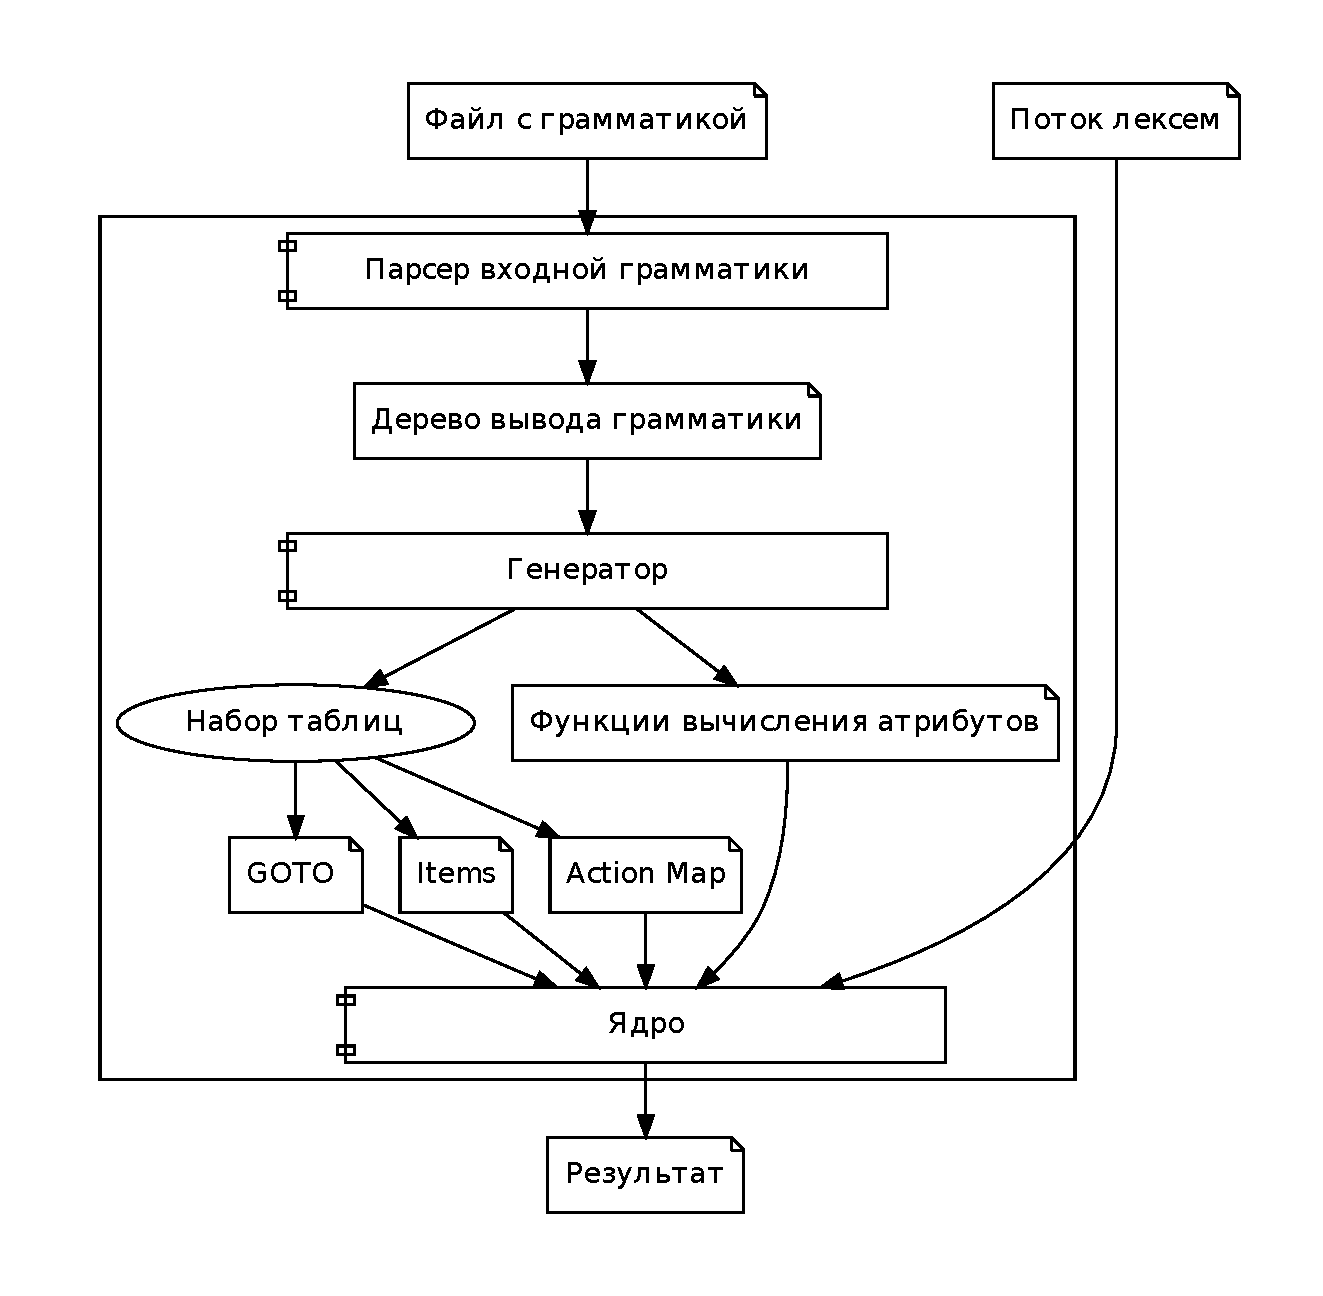
\includegraphics[height = 14.5cm]{general_tool_structure.pdf}
	\captionof{figure}{Общая структура инструмента}
	\label{fig:general_tool_structure}
\end{center}

Реализованный инструмент состоит из трёх основных модулей:
\begin{itemize}
	\item {\bfseries Парсер входной грамматики} (фронтенд), который основан на инструменте YARD, из которого используется входной язык (соответственно лексический и синтаксический анализаторы этого языка), внутреннее представление языка описания грамматики и набор преобразований (используется в генераторе). 
	
	\item {\bfseries Генератор}, который по дереву грамматики строит набор таблиц и генерирует функции для вычисления пользовательских атрибутов. Основные этапы:
		\begin{itemize}
			\item {\bfseries Преобразования грамматики}, которые необходимы, так как на уровне входного языка YARD поддерживает конструкции, которые на текущий момент наш инструмент не поддерживает(например макроправила).
				\item {\bfseries Генерация таблиц и кода}
		\end{itemize}
		Результатами работы генератора являются:
		\begin{itemize}
			\item {\bfseries Набор таблиц}, который содержит данные, необходимые для синтаксического анализа и вычисления атрибутов и состоит из:
			\begin{itemize}
				\item {\bfseries GOTO} -- таблица переходов синтаксического анализатора;
		  	\item {\bfseries Items} -- информация о состояниях  синтаксического анализатора;
		  	\item {\bfseries Action Map} -- отображение из правил в функции,  сгенерированные по атрибутам этого правила;
			\end{itemize}
			
		  \item {\bfseries Функции вычисления атрибутов } -- файл на F\#, содержащий функции для вычисления пользовательских атрибутов.
		\end{itemize}
		
		
	\item {\bfseries Ядро}, которое реализует синтаксический разбор и вычисление атрибутов и содержит:
		\begin{itemize}
			\item {\bfseries Интерпретатор таблиц}, который строит лес вывода входного выражения на основе сгенерированных таблиц. Основан на рекурсивно-восходящем алгоритме. Возвращает лес -- список деревьев вывода.
			\item {\bfseries Вычислитель атрибутов}, который обходит лес, полученный от интерпретатора таблиц, и применяет функции, найденные с помощью Action Map в сгенерированном файле, к узлам дерева.
		\end{itemize}
		
\end{itemize}

На вход поступает файл с грамматикой, заданной пользователем и поток лексем. На выходе -- результат вычислений, заданных пользователем в атрибутах грамматики.
